\section{Theory}
\label{sec:theory}

\fboxsep=1mm%padding thickness
\fboxrule=1pt%border thickness

\begin{figure*}[!ht]
	\centering
	\begin{subfigure}{0.27\linewidth}
		%  trim={<left> <lower> <right> <upper>}
        %\fcolorbox{red}{yellow}{
            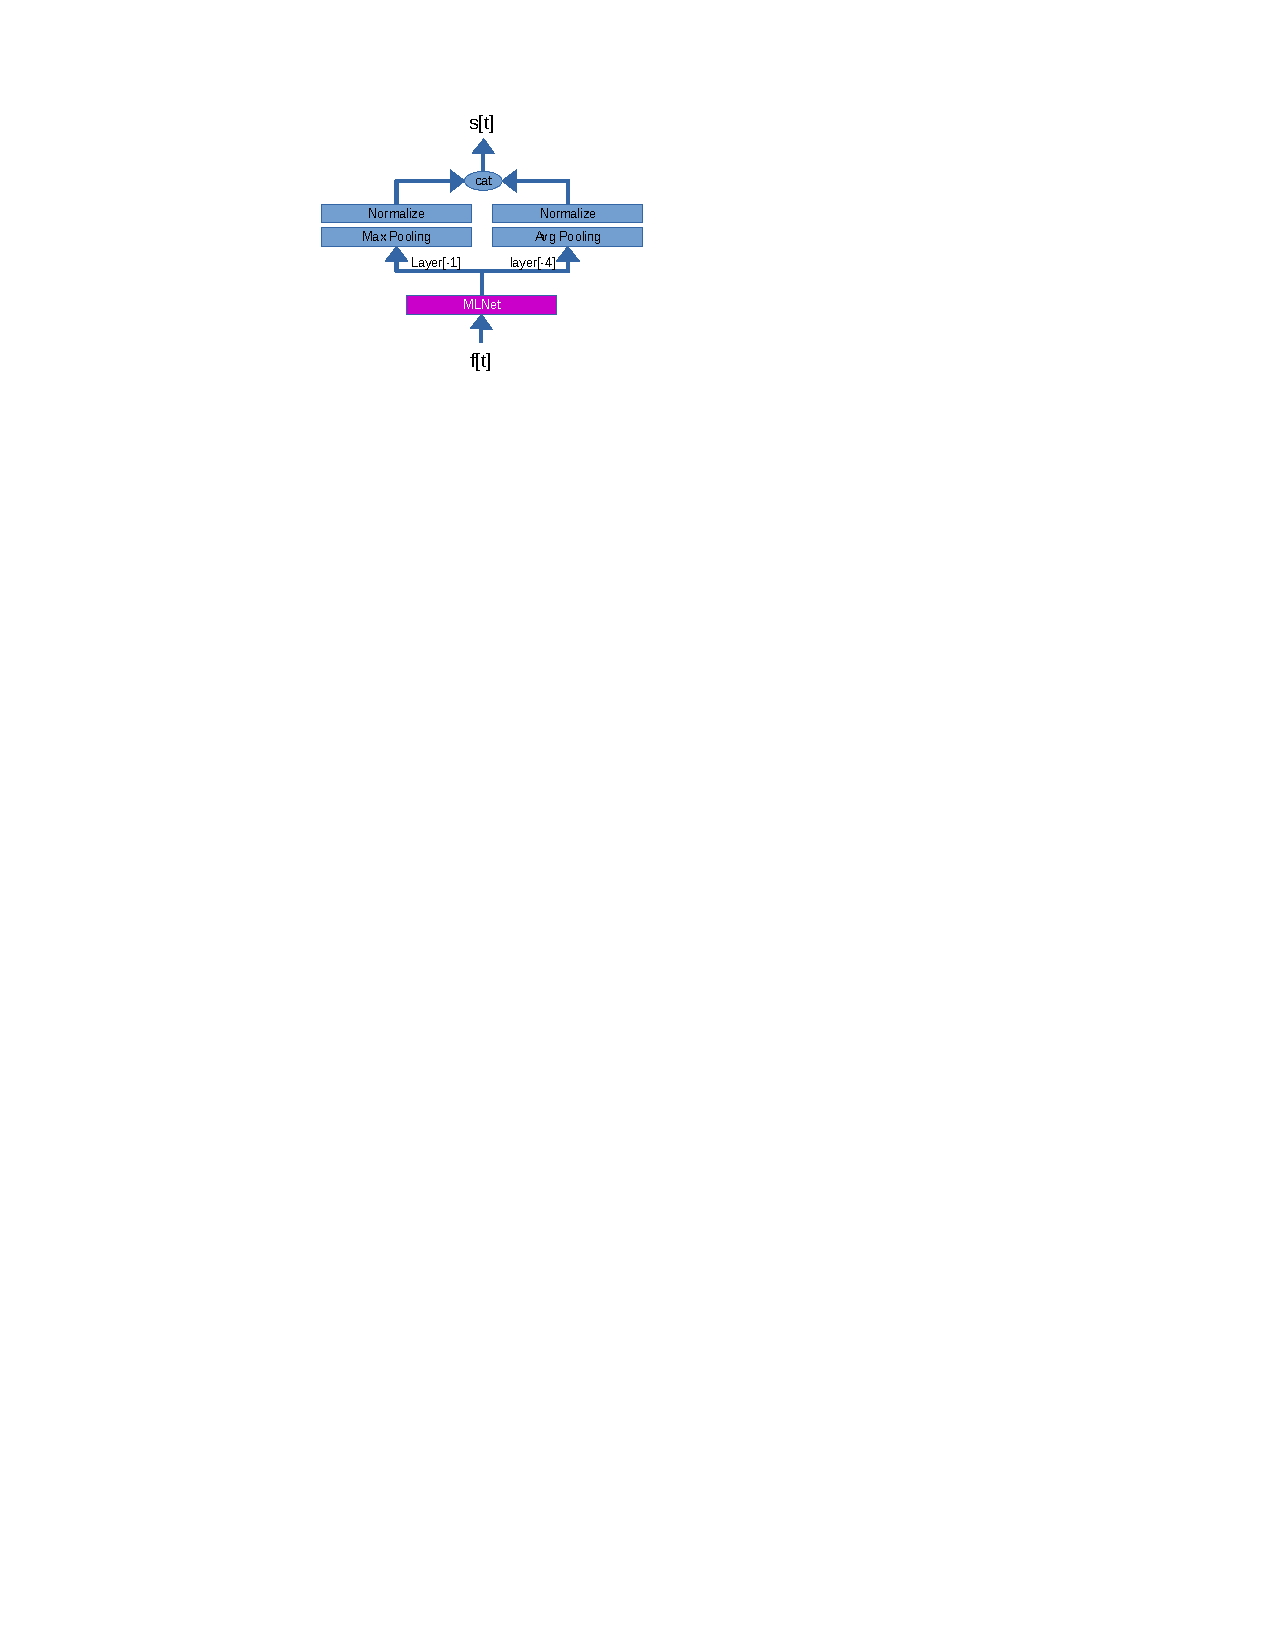
\includegraphics[trim=140 580 300 50, clip, width=1.\linewidth]{images/saliency.pdf}
        %}
        \caption{Saliency module architecture.}
        \label{fig:arch-saliency}
	\end{subfigure}
	\begin{subfigure}{0.7\linewidth}
		%  trim={<left> <lower> <right> <upper>}
        %\fcolorbox{red}{yellow}{
            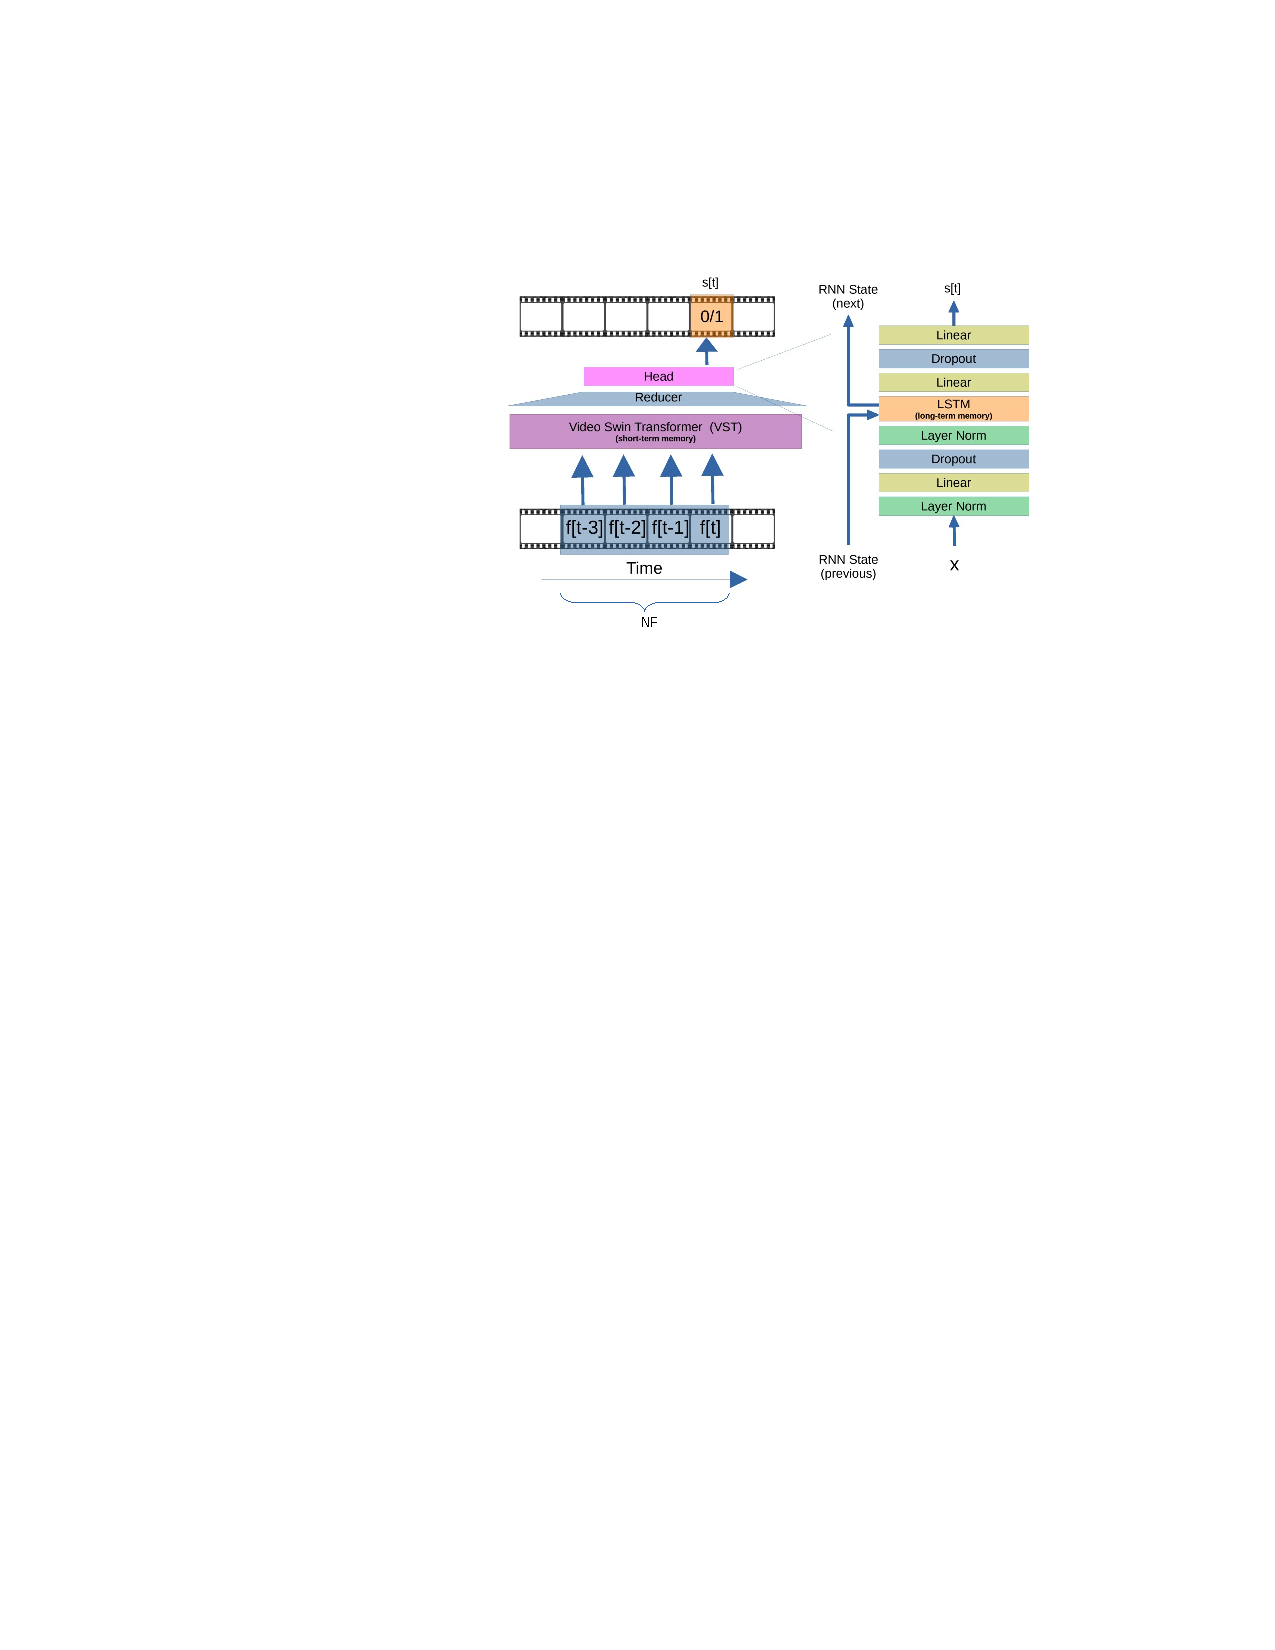
\includegraphics[trim=205 500 80 130, clip, width=1.\linewidth]{images/arch.pdf}
        %}
        % FIXME aggiungi link per immagine dei frame (copyright)
        \caption{Our online video frame anomaly detection architecture.}
		\label{fig:arch}
	\end{subfigure}
	\caption{On left the saliency module architecture more in details. On right the overall architecture.}
	\label{fig:our-arch}
\end{figure*}

In this section, the overall architecture shown in Figure \ref{fig:arch} will be exposed.
The final architecture and training modality are very simple and straightforward.
It is composed by four main blocks: a short-term memory module to encode the information related to what is happened just now, a long-term memory module to keep track of the past, a saliency module to increase the relevant information about the current frame scene and the final classification module trained to classify the current frame.
% TODO descrivere la nuova annotazione ??? Check motivazioni! :)

\subsection{Short-term memory}

Since the task provides an online frame classification, the only information available are the current and the past frames.
Our module has to deal with the current frame and the most recent ones (last three, in this case) in the most appropriate way.
Since the frames are all available by the time they are evaluated, we chosen a Transformer model instead of an RNN model due to its ability to process all of them in parallel.
In particular, the Video Swin Transformer (VST) \cite{liu_video_2022} was chosen as the base model due to its superior performance compared to a vanilla ViT \cite{DBLP:conf/iclr/DosovitskiyB0WZ21} model.
The VST model is the extension to video of the Swin Transformer \cite{liu2021Swin}, which is a general-purpose image backbone with high performance on tasks that involve detection and localization.
Originally born to carry out the task of video action classification, it has been adapted to detect anomalies on single frame in a near-real time fashion, considering a temporal window of the latest three frames at time $t_{i-2}$, $t_{i-1}$ and $t_{i}$.

The VST takes in input a video with size $T \times H \times W \times 3$, where $T$, $H$ e $W$ correspond to number of frames, height, width and channels RGB, respectively.
The model internally split the frames in non-overlapping 3D patches, partitioning the video in $\frac{T}{2} \times \frac{H}{4} \times \frac{W}{4}$ 3D tokens, projecting the features to an arbitrary dimension $C$.
The rest of the architecture is similar to Swin Transformer, with four stages of Video Swin Transformer block, interspersed with $2\times$ spatial downsampling in the patch merging layer.

As shown in Figure \ref{fig:arch}, the input of the VST is formed by $f[t_{i-2}]$, $f[t_{i-1}]$, which are buffered past frames at times $t-2$ and $t-1$, and the current frame at time $t$, respectively.

\subsection{Long-term memory}

In order to not lose information from the distant past, we needed a way to keep track of it.
Because the model is working in a online fashion, this time the requirement is opposite compared to the short-term memory.
We can only update the long-term memory sequentially, when a new frame is available.
For this reason, our choice fell on an RNN module (LSTM in this specific case) instead of a Transformer.
Its hidden state $h_t$ and cell state $c_t$ encode information about the past.
Because it doesn't need to access the past frames again but only to the latent features, the module is very efficient and lead to a limited additional computational cost.
it condenses all its knowledge into these two states.
The output of the first Linear layer of the classifier head provides the summary about the three frames processed by the short-term memory model.
Here, we added the LSTM cells which update the memory states with the new information.

\subsection{Saliency model}

Taking inspiration from DRIVE \cite{bao2021drive}, we added more information about the scene present in the current frame with the help of a saliency model, used in evaluation mode.
We adopted a VGG-16-based MLNet \cite{cornia2016deep} as saliency module, pre-trained on the fixation data of the DADA-2000 \cite{fang2019dada} training set, with the parameters frozen during the new training.

As seen in the Figure \ref{fig:arch-saliency}, we normalized and concatenated the output of MLNet last layer and the fourth last layer, to form a single saliency vector $s[t]$ of 2275 values.
Before the concatenation, the features are passed through a max pooling and average pooling, respectively.

\subsection{Classification module (Head)}

After reducing the output of the VST with a Adaptive Average Pool 3D (Reducer), the classification module process it generating the anomaly classification score for the current frame.
As shown in Figure \ref{fig:arch}, the head is composed by some Linear layers, the LSTM cells and the branch connected with the saliency module.
The final output is the anomaly classification score of the current frame at time $t$.
This is trained with a weighted cross-entropy loss, giving more weight to the anomaly class, because it is spotted less frequently.

% copyright image frame: <a href="https://www.freepik.com/free-vector/realistic-vector-icon-film-tape-strip-with-white-square-isolated-white-cinema-concept_31096470.htm#query=video%20frame&position=31&from_view=keyword">Image by user15245033</a> on Freepik